\documentclass[a4paper, 12pt]{article}

\newcommand{\templates}{../../template}
\usepackage[a4paper, margin=2.5cm]{geometry}

\usepackage{enumitem}
\setlist[itemize]{noitemsep}
\setlist[enumerate]{noitemsep}

\let\oldpar\paragraph
\renewcommand{\paragraph}[1]{\oldpar{#1\\}\noindent}
\usepackage{graphicx}
\usepackage{hyperref}
\usepackage{makecell}

\newcommand{\settitolo}[1]{\newcommand{\titolo}{#1\\}}
\newcommand{\setprogetto}[1]{\newcommand{\progetto}{#1\\}}
\newcommand{\setcommittenti}[1]{\newcommand{\committenti}{#1\\}}
\newcommand{\setredattori}[1]{\newcommand{\redattori}{#1\\}}
\newcommand{\setrevisori}[1]{\newcommand{\revisori}{#1\\}}
\newcommand{\setresponsabili}[1]{\newcommand{\responsabili}{#1\\}}
\newcommand{\setversione}[1]{
	\ifdefined\versione\renewcommand{\versione}{#1\\}
	\else\newcommand{\versione}{#1\\}\fi
}
\newcommand{\setdestuso}[1]{\newcommand{\uso}{#1\\}}
\newcommand{\setdescrizione}[1]{\newcommand{\descrizione}{#1\\}}

\newcommand{\makefrontpage}{
	\begin{titlepage}
		\begin{center}

		
\includegraphics[width=0.4\textwidth]{../../template/WSWS-logos_transparent_crop}\\

		{\Large Winning Software Solution}\\[6pt]
		\href{mailto://winningsoftwaresolution@gmail.com}{winningsoftwaresolution@gmail.com}\\
		
		\ifdefined\progetto
		\vspace{1cm}
		{\Large\progetto}
		{\large\committenti}
		\else\fi
		
		\vspace{1.5cm}
		{\LARGE\titolo}
		
		\vfill
		
		\begin{tabular}{r | l}
		\multicolumn{2}{c}{\textit{Informazioni}}\\
		\hline
		
		\ifdefined\redattori
			\textit{Redattori} &
			\makecell[l]{\redattori}\\
		\else\fi
		\ifdefined\revisori
			\textit{Revisori} &
			\makecell[l]{\revisori}\\
		\else\fi
		\ifdefined\responsabili
			\textit{Respondabili} &
			\makecell[l]{\responsabili}\\
		\else\fi
		
		\ifdefined\versione
			\textit{Versione} & \versione
		\else\fi
		
		\textit{Uso} & \uso
		
		\end{tabular}
		
		\vspace{2cm}
		
		\ifdefined\descrizione
		Descrizione
		\vspace{6pt}
		\hrule
		\descrizione
		\else\fi
		\end{center}
	\end{titlepage}
}
\usepackage{hyperref}
\usepackage{array}
\usepackage{tabularx}

\def\vers#1-#2-#3-#4-#5\\{#1&#2&#3&#4&#5\\\hline}

\newcommand{\addversione}[5]{
	\ifdefined\versioni
		\let\old\versioni
		\renewcommand{\versioni}{#1&#2&#3&#4&#5\\\hline\old}
	\else
		\newcommand{\versioni}{#1&#2&#3&#4&#5\\\hline}
	\fi
}

\newcommand{\setversioni}[1]{\newcommand{\versioni}{#1}}

\newcommand{\makeversioni}{
	\begin{center}
		\begin{tabularx}{\textwidth}{|c|c|c|c|X|}
		\hline
		\textbf{Versione} & \textbf{Data} & \textbf{Persona} & \textbf{Attivtà} & \textbf{Descrizione} \\
		\hline
		\versioni
		\end{tabularx}
	\end{center}
	\clearpage
}
\usepackage{hyperref}
\usepackage{graphicx}
\usepackage{placeins}
\usepackage{listings}
\settitolo{Manuale Sviluppatore Shop Chain}
\setredattori{WinningSoftwareSolution}
\setdestuso{esterno}
\setdescrizione{
Manuale sviluppatore.
}

\addversione{0.1.0}{04/04/2022}{Federico Marchi}{Redazione}{Stesura iniziale}
\addversione{1.0.0}{07/05/2022}{Federico Marchi}{Redazione}{Stesura finale}

\begin{document}
\makefrontpage

\makeversioni

\tableofcontents
\newpage

\section{Introduzione}
\label{sec:intro}
Il presente documento ha la funzione di descrivere in dettaglio la procedura da seguire per l'installazione di tutte le componenti necessarie per il corretto funzionamento di Shop Chain. Si garantisce il corretto funzionamento del prodotto con le versioni indicate nel documento per i software utilizzati.\\
È necessario clonare la repository GitHub al seguente indirizzo: \url{https://github.com/iota97/WinningSoftwareSolution}.\\

\newpage{}
\section{Server}
\subsection{Requisiti}
\subsubsection{Node Js}
Installare \href{https://nodejs.org/en/download/}{Node Js} (v. 16.13.1) se non è già stato installato precedentemente. Una volta effettuata correttamente l'installazione, è necessario eseguire il seguente comando direttamente nella cartella "Server" per l'installazione delle dipendenze:
\begin{lstlisting}[language=bash]
  $ npm install
\end{lstlisting}
\subsubsection{Metamask}
Per poter utilizzare la web app è necessario Metamask (v. 10.11.3).\\
Per avere il proprio wallet Metamask è possibile recarsi su \href{https://www.metamask.io}{metamask.io}, installare l'estensione e scegliere se:
\begin{itemize}
  \item \textbf{Creare un nuovo wallet}: è possibile creare un nuovo wallet selezionando "Create a Wallet" (Fig. 1 freccia blu). Durante la creazione del wallet ricordare di salvare la mnemonic phrase poiché necessaria nei passi successivi;
  \item \textbf{Importare un wallet già esistente}: è possibile anche importare un wallet già esistente selezionando l'opzione "Import wallet" (Fig. 1 freccia rossa). È sufficiente inserire la mnemonic phrase per poter utilizzare il proprio wallet su Metamask.
\end{itemize}
\FloatBarrier
\begin{figure}[!h]
\centering
\includegraphics[width=0.8\linewidth]{img/metamask.png}
\caption{Creazione/Importazione wallet su Metamask.}
\end{figure}
\FloatBarrier
\paragraph{Recupero mnemonic phrase}\\
Nel caso in cui non si ricordi più la mnemonic phrase del proprio wallet è possibile recuperarla dal proprio account Metamask con la seguente procedura:
\begin{enumerate}
  \item accedere al proprio wallet Metamask;
  \item selezionare il proprio account in alto a destra (Fig. 2);
  \item selezionare l'opzione "Settings";
  \item selezionare l'opzione "Security \& Privacy";
  \item selezionare l'opzione "Reveal Secret Recovery Phrase";
  \item inserire la propria password.
\end{enumerate}
Una volta ottenuta la propria mnemonic phrase salvarla per i passi successivi.
\FloatBarrier
\begin{figure}[!h]
\centering
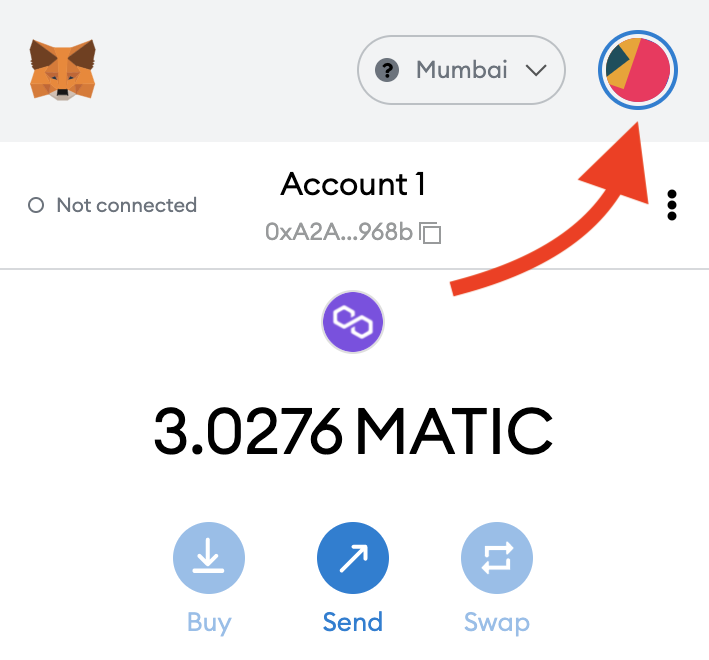
\includegraphics[width=0.4\linewidth]{img/account_meta.png}
\caption{Selezione account Metamask.}
\end{figure}
\FloatBarrier
\paragraph{Configurazione mainnet Polygon}\\
Per l'inserimento e la configurazione della rete Polygon nel proprio wallet Metamask è necessario utilizzare i seguenti dati:
\begin{itemize}
\item Network Name: \textbf{Polygon};
\item New RPC Url: \textbf{https://rpc-mainnet.matic.network};
\item ChainID: \textbf{137};
\item Currency Simbol: \textbf{MATIC};
\item Block Explorer URL: \textbf{https://polygonscan.com/}.
\end{itemize}
\paragraph{Configurazione testnet Mumbai}\\
Nel caso in cui si desidrasse operare sulla testnet Mumbai di Polygon, utilizzare i seguenti dati:
\begin{itemize}
\item Network Name: \textbf{Mumbai};
\item New RPC Url: \textbf{https://rpc-mumbai.maticvigil.com/};
\item ChainID: \textbf{80001};
\item Currency Simbol: \textbf{MATIC};
\item Block Explorer URL: \textbf{https://mumbai.polygonscan.com/}.
\end{itemize}
Nella testnet Mumbai è possibile eseguire qualsiasi operazione senza dover necessariamente spendere soldi. Infatti per rifornire il proprio wallet di MATIC di prova si può utilizzare il faucet all'indirizzo \url{https://faucet.polygon.technology/}.\\ \\
Una volta inseriti i dati e aggiunta la rete, ricordare di selezionarla.
\subsubsection{Provider}
\label{sec:provider}
Per ottenere il provider per la mainnet Polygon è necessario registrarsi su \href{https://www.moralis.io}{moralis.io}. Una volta effettuata la registrazione:
\begin{enumerate}
  \item selezionare la sezione "SpeedyNodes" dal menù;
  \item selezionare l'endpoint per Polygon Network;
  \item selezionare il protocollo WS;
  \item copiare l'url dell'endpoint per la mainnet (Fig. 3 freccia rossa).
\end{enumerate}
Nell'url copiato è possibile visualizzare l' api key, si tratta infatti del codice evidenziato in grassetto nel seguente esempio:\\\\
wss://speedy-nodes-nyc.moralis.io/\textbf{a8d734a415dd368a3498db63}/polygon/mainnet/ws\\\\
È necessario salvare l'url per i passi successivi.
\paragraph{Testnet Mumbai}\\
Nel caso in cui si volesse invece utilizzare una rete di test, è possibile utilizzare la rete Mumbai la quale è una testnet di Polygon. Per selezionare il provider corretto per Mumbai è sufficiente copiare l'url nel campo "Mumbai" (Fig. 3 freccia blu).
\FloatBarrier
\begin{figure}[!h]
\centering
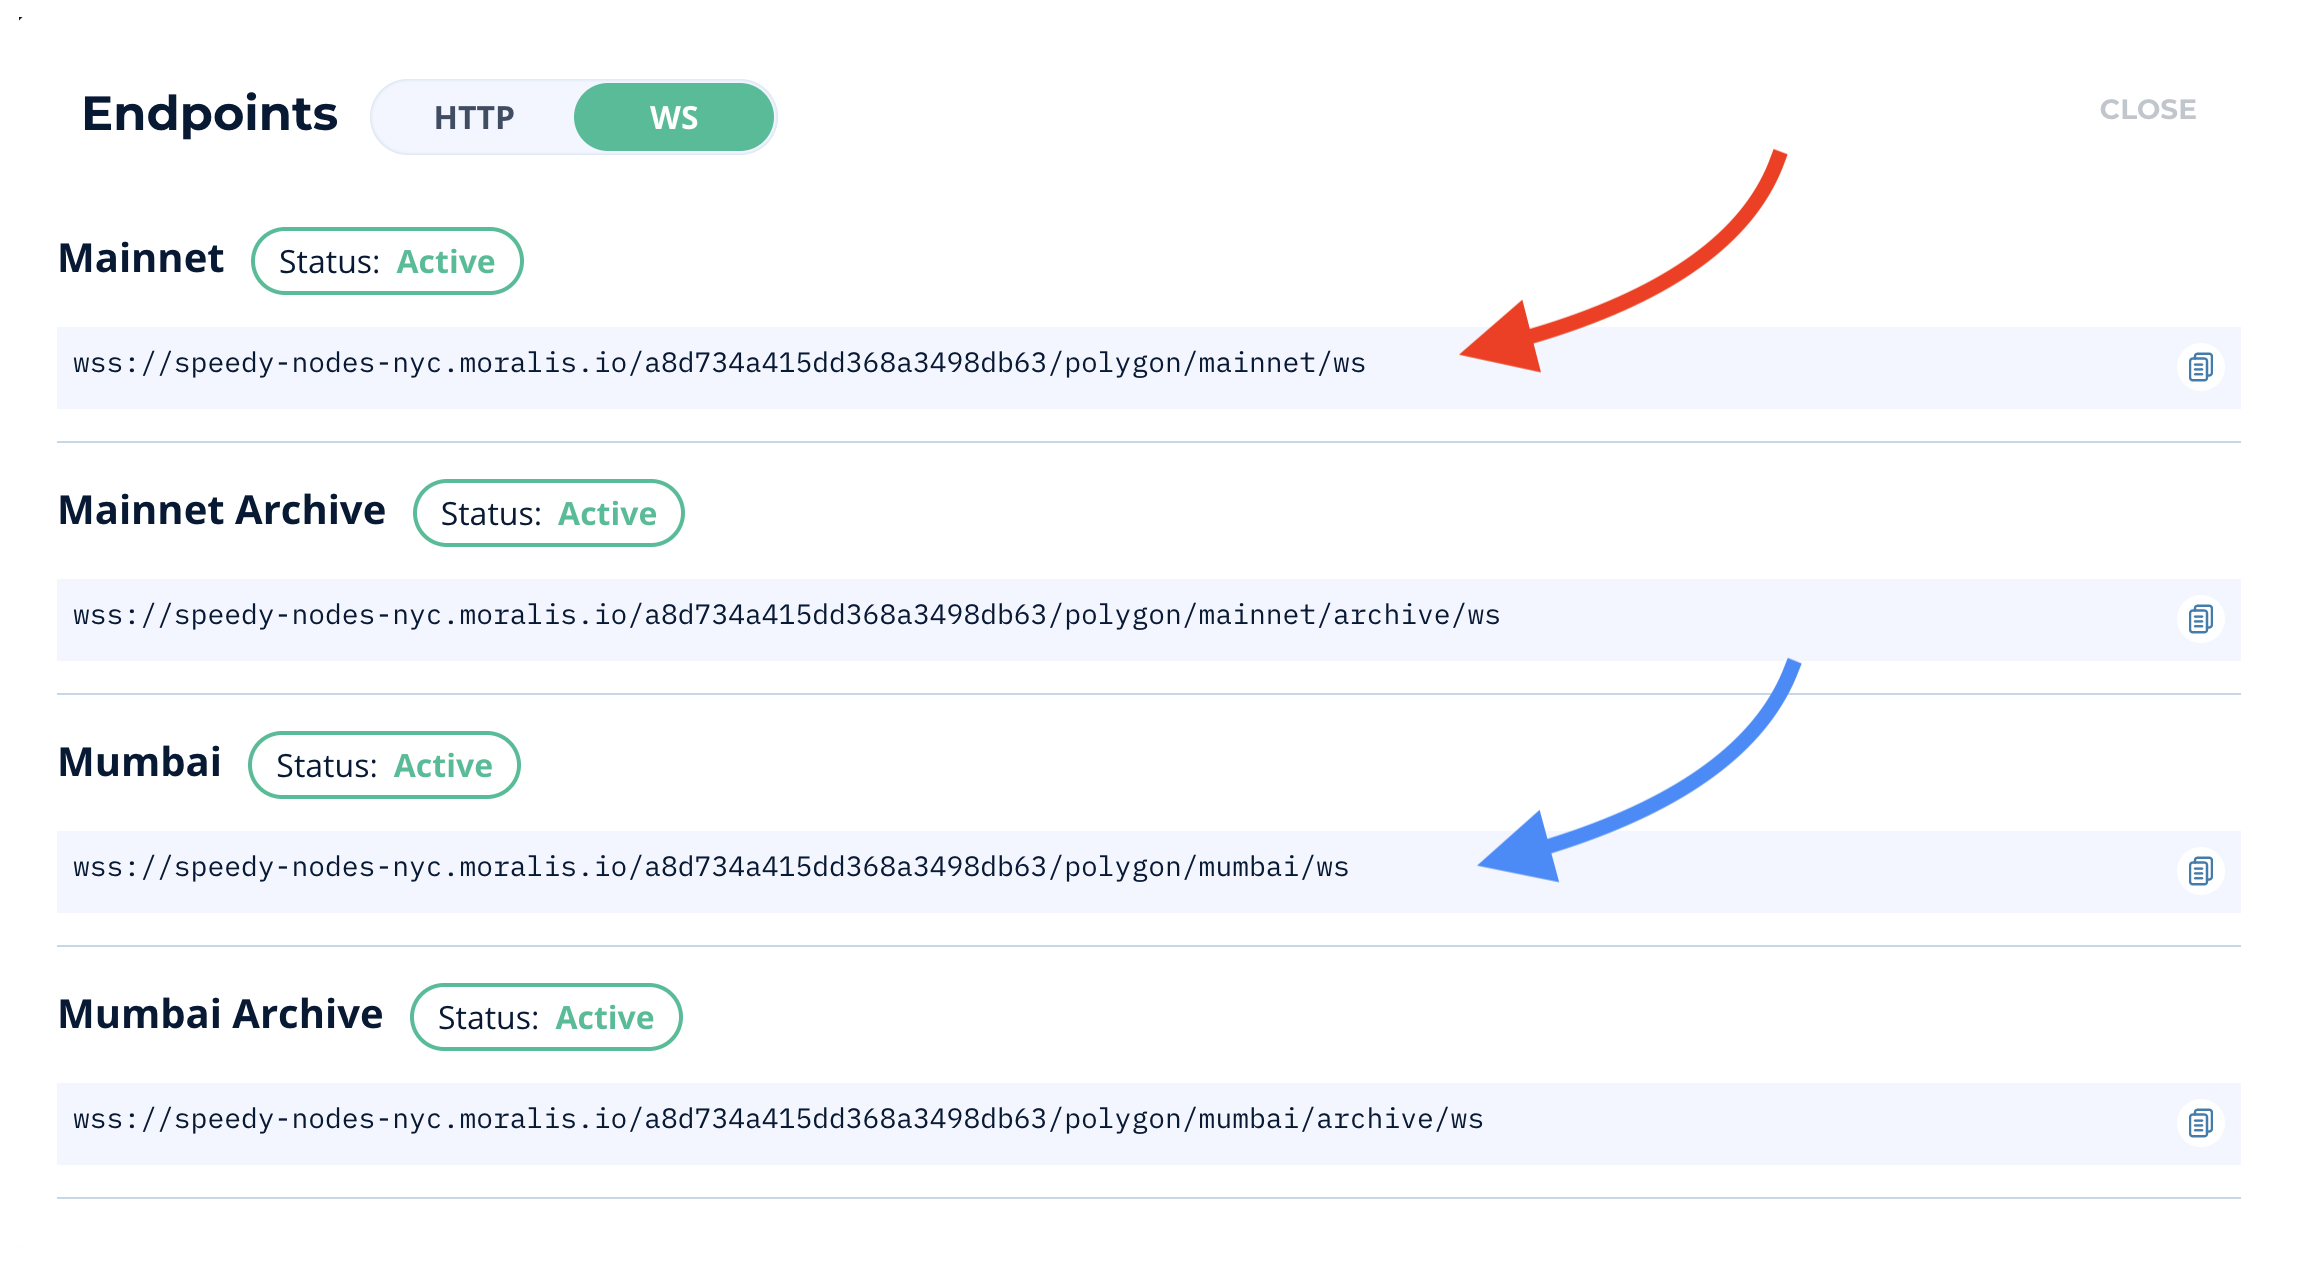
\includegraphics[width=0.6\linewidth]{img/moralis.png}
\caption{Provider su moralis.io.}
\end{figure}
\FloatBarrier
\subsubsection{MariaDB}
\label{sec:db}
Installare il database \href{https://mariadb.org/download/}{MariaDB} (v. 10.7.3) se non è già stato installato precedentemente. Una volta eseguita l'installazione del database, collegarsi con il comando:
\begin{lstlisting}[language=bash]
  $ sudo mysql -u <user> -p <password>
\end{lstlisting}
e sostituire:
\begin{itemize}
  \item \verb|<user>|: con l'user con il quale si desidera creare il database;
  \item \verb|<password>|: con la password dell'user selezionato.
\end{itemize}
Effettuato il collegamento eseguire la seguente query per la creazione del database:
\begin{verbatim}
CREATE DATABASE OnlineStore;
\end{verbatim}
Successivamente creare le tabelle con le seguenti query:
\begin{verbatim}
USE OnlineStore;
DROP TABLE PaymentEntries;
DROP TABLE SettledPayments;
DROP TABLE LastBlockSynced;
CREATE TABLE PaymentEntries (id bigint, ecommerce varchar(255) not null,
price bigint not null, primary key(id));
CREATE TABLE SettledPayments (id bigint, item_id bigint not null,
buyer varchar(255) not null, status int not null, created bigint not null,
confirmed bigint, primary key(id));
CREATE TABLE LastBlockSynced (id int(1), value bigint not null, primary key(id));
INSERT INTO LastBlockSynced (id, value) VALUES (0, 0);
\end{verbatim}
\subsection{Configurazione}
\label{sec:config_server}
Una volta clonata la repository come spiegato nell'\hyperref[sec:intro]{introduzione}, è necessaria la creazione di un file `.env` dentro la cartella "Server". Il file deve essere strutturato come segue:
\begin{verbatim}
  PORT=8080
  DB_HOST="localhost"
  DB_USER="username"
  DB_PWD="password"
  DB_NAME="OnlineStore"
  API_KEY=xxxxxxxxxxxxxxxxxxxxxxxx
  SERVER_URL="tinyurl.com/xxxxxxxx"
\end{verbatim}
dove ciascun campo indica:
\begin{itemize}
  \item \textbf{PORT}: la porta che si desidera utilizzare;
  \item \textbf{DB\_HOST}: l'host selezionato;
  \item \textbf{DB\_USER}: l'user associato al database;
  \item \textbf{DB\_PWD}: password dell' user utilizzato;
  \item \textbf{DB\_NAME}: il nome del database da utilizzare, in questo caso "OnlineStore";
  \item \textbf{API\_KEY}: l' api key, ottenibile come spiegato al punto \hyperref[sec:provider]{2.1.2}.
  \mbox{}
  \item \textbf{SERVER\_URL}: inserire il link ritornato da localtunnel come spiegato nel seguente paragrafo.\\
  \paragraph{Sviluppo e testing con Localtunnel}\\
  Per lo sviluppo e il testing è stato utilizzato il tool localtunnel, il quale permette di rendere accessibile da remoto il server locale. Per utilizzare localtunnel è necessario:
  \begin{itemize}
    \item eseguire l'installazione globalmente con il comando:
    \begin{lstlisting}[language=bash]
      $ npm install -g localtunnel
    \end{lstlisting}
    \item avviare localtunnel con il comando:
    \begin{lstlisting}[language=bash]
      $ lt --port <port>
    \end{lstlisting}
    con \verb|<port>| la porta che si desidera utilizzare (deve corrispondere con la porta specificata nella variabile d'ambiente \verb|PORT|);\\
    \item il link ritornato inserirlo nella variabile d'ambiente \verb|SERVER_URL|. Importante ricordarsi di aggiornare il link ogni qualvolta si riavvia localtunnel.
  \end{itemize}

\end{itemize}
\subsection{Avvio server e test}
\label{sec:avvio}
Conclusa la configurazione è possibile far partire il server con il comando:
\begin{lstlisting}[language=bash]
  $ npm start
\end{lstlisting}
Mentre per i test è sufficiente la creazione del database "OnlineStoreTest" inserendo le seguenti query come spiegato al punto \hyperref[sec:db]{2.1.3}:
\begin{verbatim}
CREATE DATABASE OnlineStoreTest;
USE OnlineStoreTest;
DROP TABLE PaymentEntries;
DROP TABLE SettledPayments;
DROP TABLE LastBlockSynced;
CREATE TABLE PaymentEntries (id bigint, ecommerce varchar(255) not null,
price bigint not null, primary key(id));
CREATE TABLE SettledPayments (id bigint, item_id bigint not null,
buyer varchar(255) not null, status int not null, created bigint not null,
confirmed bigint, primary key(id));
CREATE TABLE LastBlockSynced (id int(1), value bigint not null, primary key(id));
INSERT INTO LastBlockSynced (id, value) VALUES (0, 0);
\end{verbatim}
e successivamente eseguire il comando:
\begin{lstlisting}[language=bash]
  $ npm test
\end{lstlisting}
\subsection{Test sulla Web App}
Per eseguire i test sulla web app si utilizza JSCover in modalità proxy. I file Javascript della web app passano attraverso un server proxy che li trasforma e tiene traccia della loro copertura. Per eseguire correttamente il test seguire la seguente procedura:
\begin{itemize}
  \item avviare il server di Shop Chain come spiegato al punto \hyperref[sec:avvio]{2.3};
  \item avviare il server proxy con il comando:
  \begin{lstlisting}[language=bash]
    $ java -jar JSCover-all.jar -ws --proxy --port=3128
    --report-dir=jscoverage --local-storage
  \end{lstlisting}
  è possibile cambiare porta nel caso la porta \verb|3128| sia già occupata;
  \item configurare il proxy aggiungendo come host \verb|localhost-proxy| e impostare come proxy \verb|localhost-proxy:3128|;
  \item per eseguire i test è necessario connettersi a \url{http://localhost-proxy:8080}.
\end{itemize}
\paragraph{Salvataggio dati}\\
JScover tiene traccia di ogni linea di codice eseguita e salva i dati nel localStorage di HTML5. Per salvare i dati nella cartella "jscoverage" è necessario:
\begin{itemize}
  \item caricare la pagina \url{http://localhost-proxy:8080/jscoverage.html};
  \item aprire la tab "Store";
  \item selezionare "Store Report".
\end{itemize}
\paragraph{Cancellazione dati}\\
Essendo i dati dei test cumulativi, quando si desidera effettuare il test da zero è necessario cancellare i dati salvati. Per la cancellazione dei dati è sufficiente caricare la pagina \url{http://localhost-proxy:8080/jscoverage-clear-local-storage.html}.
\paragraph{Visualizzazione report}\\
Per la visualizzazione del report è sufficiente selezionare la tab "Summary" nella seguente pagina:  \url{http://localhost-proxy:8080/jscoverage-clear-local-storage.html}.
\newpage{}
\section{Script}
Lo script in python permette all'e-commerce di creare una istanza di pagamento in blockchain e dunque permettere all'acquirente di acquistare attraverso il servizio Shop Chain.
\subsection{Requisiti}
\subsubsection{Python e dipendenze}
Al fine di utilizzare correttamente lo script è necessario:
\begin{itemize}
  \item \href{https://www.python.org/downloads/}{python3.8};
  \item pip3.8;
  \item installare le seguenti dipendenze con i comandi:
  \begin{lstlisting}[language=bash]
    $ pip3.8 install web3
    $ pip3.8 install python-dotenv
    $ pip3.8 install pytest
  \end{lstlisting}
\end{itemize}
\subsection{Configurazione}
È necessario creare un file chiamato `.env` all'interno della stessa cartella contenente lo script \textit{sell.py}. Il file dovrà contenere:
\begin{itemize}
  \item la mnemonic phrase del proprio wallet;
  \item il provider ottenuto al punto \hyperref[sec:provider]{2.1.2}.
\end{itemize}
Di seguito un esempio del formato corretto da utilizzare:
\begin{verbatim}
MNEMONIC=mnemonic phrase del proprio wallet
PROVIDER=provider url
\end{verbatim}
\subsection{Creazione di un'istanza di pagamento}
Una volta soddisfatti i requisiti e ultimata la configurazione è possibile procedere con l'esecuzione dello script python per la creazione di un'istanza di pagamento. Verranno illustrati due modi per la corretta esecuzione dello script \textit{sell.py}.
\subsubsection{Sell.py da terminale}
È possibile eseguire lo script \textit{sell.py} direttamente da terminale, attraverso il comando:
\begin{lstlisting}[language=bash]
  $ python3 sell.py [item price]
\end{lstlisting}
Sostituire \verb|[item price]| con il prezzo con il quale si creare l'istanza di pagamento.
Una volta eseguito lo script, verrà ritornato e stampato l'id e il prezzo dell'istanza creata.
\textbf{Esempio}
\\
Se vogliamo vendere un prodotto al prezzo di 2\$, basterà inviare il comando:
\begin{lstlisting}[language=bash]
  $ python3 sell.py 2
\end{lstlisting}
l'output visualizzato sarà:
\begin{lstlisting}[language=bash]
  $ [Adding] Price: 2
  $ [Added] Payment entry id: 3, price: 2
\end{lstlisting}
Dove :
\begin{itemize}
  \item \textbf{paymement entry id: 3}: indica che l'id dell'oggetto messo in vendita è 3;
  \item \textbf{price: 2}: indica che il prezzo a cui è stato messo in vendita il prodotto è di 2\$.
\end{itemize}
\subsubsection{Script python}
È possibile includere un proprio script in python nel backend dell' e-commerce per permettere direttamente la creazione delle istanze per i pagamenti.\\
La funzione che viene utilizzata è \textbf{sell\_item} di \textit{sell.py}. La funzione richiede in input un solo parametro, ovvero il prezzo in dollari che si desidera assegnare all'istanza di pagamento.\\
È dunque necessario includere nel proprio script la funzione come segue:
\begin{verbatim}
from sell import sell_item
\end{verbatim}
\subsection{Reindirizzamento alla landing page}
Al fine di permettere all'acquirente, direttamente dal proprio e-commerce, di essere reindirizzato sulla landing page di Shop Chain per effettuare l'acquisto è necessario strutturare l'url di reindirizzamento come segue:
\begin{quote}
  \verb|\land?id=<id_item>&r=<pagina_di_ritorno>|.
\end{quote}
e dunque sostituire:
\begin{itemize}
  \item \verb|<id_item>| con l'id dell'istanza che si riferisce all'acquisto che l'acquirente desidera effettuare;
  \item \verb|<pagina_di_ritorno>| con l'url della pagina alla quale si vuole reindirizzare l'acquirente al termine dell'acquisto.
\end{itemize}
Dopo aver confermato il pagamento l'acquirente verrà direttamente reindirizzato alla pagina di ritorno, l'url sarà strutturato come segue:
\begin{quote}
  \verb|<pagina_di_ritorno>?transaction_id=<id_transazione>|.
\end{quote}
dove \verb|<id_transazione>| corrisponde all'id della transazione effettuata dall'acquirente per l'acquisto.
\end{document}
\subsection{Test}
Per eseguire il test sullo script è sufficiente eseguire il seguente comando:
\begin{lstlisting}[language=bash]
$ pytest
\end{lstlisting}
\section{Contract}
\subsection{Requisiti}
\subsubsection{Truffle, plugin e librerie}
Per compilare lo smart contract e deployarlo è necessario installare Truffle e alcuni plugin e librerie all'interno della cartella "Contract". Eseguire i seguenti comandi per una corretta installazione:
\begin{lstlisting}[language=bash]
  $ npm install
  $ npm install -g truffle
  $ npm install @truffle/hdwallet-provider
\end{lstlisting}
per le librerie eseguire:
\begin{lstlisting}[language=bash]
  $ npm install @openzeppelin/contracts
  $ npm install @chainlink/contracts
\end{lstlisting}
infine per la verifica e test installare:
\begin{lstlisting}[language=bash]
  $ npm install truffle-plugin-verify
  $ npm install solidity-coverage
\end{lstlisting}
\subsection{Configurazione}
È necessaria la creazione di tre file nella cartella "Contract" per il deployment del contratto:
\begin{itemize}
  \item \textbf{mnemonic.secret}: deve contenere la mnemonic del proprio wallet;
  \item \textbf{providerlink.secret}: deve contenere l'url del provider ottenibile come spiegato al punto \hyperref[sec:provider]{2.1.2}, può essere utilizzato anche l'url in http;
  \item \textbf{apikey.secret}: deve contenere l' api key necessaria per la verifica del contratto. Per ottenere l'api key registrarsi su \href{https://polygonscan.com/}{PolygonScan}, una volta eseguita la registrazione andare al seguente url per generare la propria api key: \url{https://polygonscan.com/myapikey}.
\end{itemize}
\subsection{Compilazione, deployment e verifica}
\paragraph{Compilazione}\\
Per la compilazione del contract è sufficiente eseguire il seguente comando:
\begin{lstlisting}[language=bash]
  $ truffle compile
\end{lstlisting}
\paragraph{Deployment}\\
Per il deployment del contratto eseguire il seguente comando:
\begin{lstlisting}[language=bash]
  $ truffle deploy --network <YOUR_NETWORK>
\end{lstlisting}
dove \verb|<YOUR_NETWORK>| rappresenta il network che si desidera utilizzare, in questo caso viene utilizzato \verb|polygon_mumbai|. Il network è definito nel file \textit{truffle-config.js}.\\ \\
In caso di errori di timeout cambiare l'url nel file \textit{providerlink.secret} da http a wss e/o eseguire il comando aggiungendo:
\begin{lstlisting}[language=bash]
  $ truffle deploy --network <YOUR_NETWORK> --reset --compile-none
\end{lstlisting}
A questo punto è necessario registrare l'upkeeper di ChainLink per il proprio contratto al fine di poter utilizzare un timer per la scadenza degli ordini. Registrarsi dunque su \url{https://keepers.chain.link/} e seguire la procedura illustrata nella documentazione di ChainLink al seguente url: \url{https://docs.chain.link/docs/chainlink-keepers/register-upkeep/}.
\paragraph{Verifica}\\
Per la verifica del contratto eseguire il comando:
\begin{lstlisting}[language=bash]
  $ truffle run verify ShopContract --network <YOUR-NETWORK>
\end{lstlisting}
questo comando ritorna un link a PolygonScan nel quale è possibile visualizzare il codice verificato e le ABI del contratto.
\subsection{Test}
Per testare senza copertura del codice eseguire il comando:
\begin{lstlisting}[language=bash]
  $ truffle test --network <YOUR-NETWORK> ./test/shopcontract.js
\end{lstlisting}
mentre per testare con copertura del codice eseguire il comando:
\begin{lstlisting}[language=bash]
  $ sudo truffle run coverage --file="./test/shopcontract.js"
    --solcoverjs ./.solcover.js
\end{lstlisting}
\end{document}
